% Created by tikzDevice version 0.6.2 on 2012-04-24 14:14:48
% !TEX encoding = UTF-8 Unicode
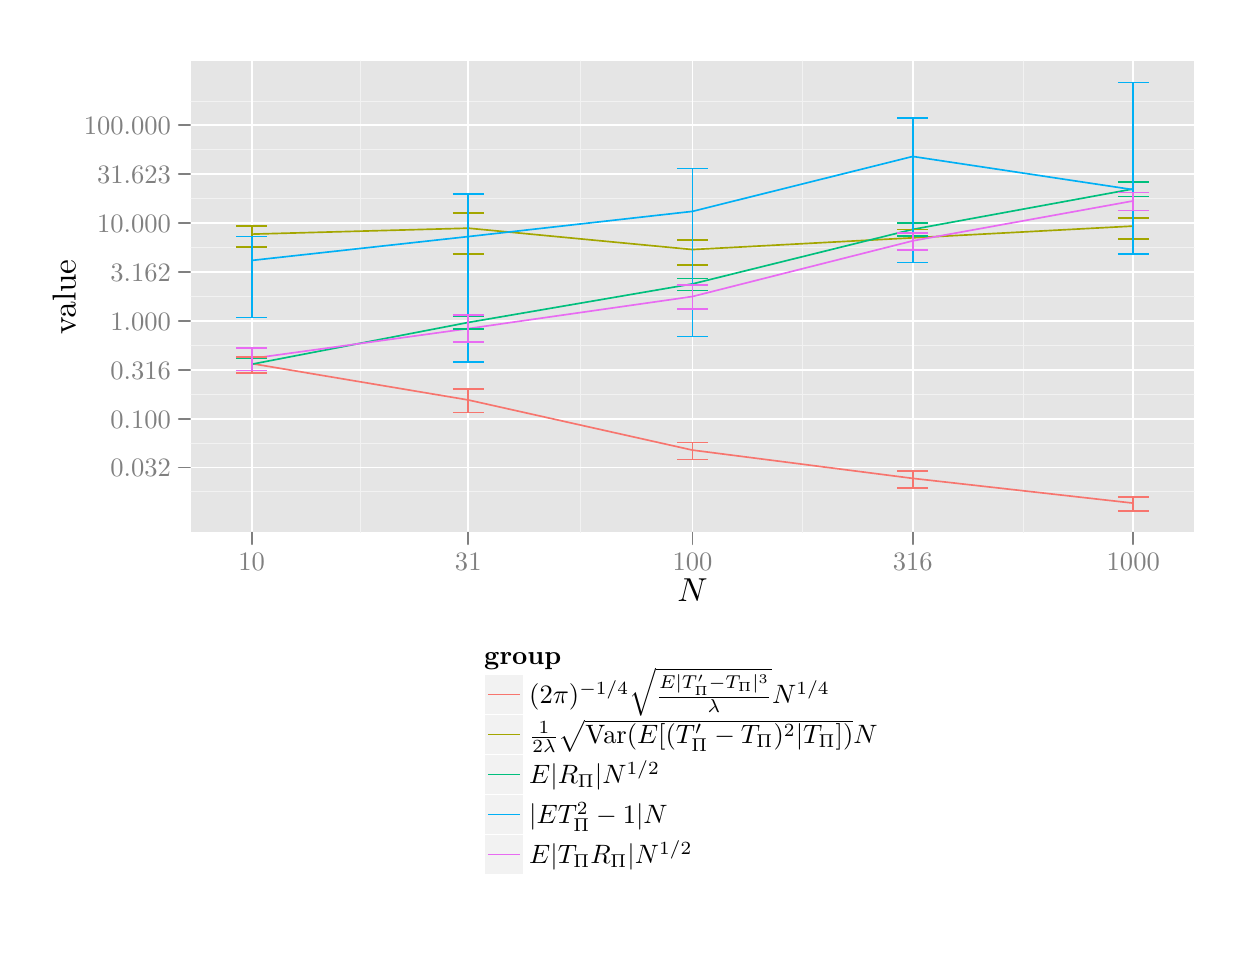
\begin{tikzpicture}[x=1pt,y=1pt]
\definecolor[named]{drawColor}{rgb}{0.00,0.00,0.00}
\definecolor[named]{fillColor}{rgb}{1.00,1.00,1.00}
\fill[color=fillColor,fill opacity=0.00,] (0,0) rectangle (433.62,325.21);
\begin{scope}
\path[clip] (  0.00,  0.00) rectangle (433.62,325.21);
\definecolor[named]{drawColor}{rgb}{0.41,0.16,0.58}
\end{scope}
\begin{scope}
\path[clip] (  0.00,  0.00) rectangle (433.62,325.21);
\definecolor[named]{drawColor}{rgb}{0.41,0.16,0.58}
\end{scope}
\begin{scope}
\path[clip] (  0.00,  0.00) rectangle (433.62,325.21);
\definecolor[named]{drawColor}{rgb}{0.41,0.16,0.58}
\end{scope}
\begin{scope}
\path[clip] (  0.00,  0.00) rectangle (433.62,325.21);
\definecolor[named]{drawColor}{rgb}{0.41,0.16,0.58}
\end{scope}
\begin{scope}
\path[clip] (  0.00,  0.00) rectangle (433.62,325.21);
\definecolor[named]{drawColor}{rgb}{0.41,0.16,0.58}
\end{scope}
\begin{scope}
\path[clip] (  0.00,  0.00) rectangle (433.62,325.21);
\definecolor[named]{drawColor}{rgb}{0.41,0.16,0.58}
\end{scope}
\begin{scope}
\path[clip] (  0.00,  0.00) rectangle (433.62,325.21);
\definecolor[named]{drawColor}{rgb}{0.41,0.16,0.58}
\end{scope}
\begin{scope}
\path[clip] (  0.00,  0.00) rectangle (433.62,325.21);
\definecolor[named]{drawColor}{rgb}{0.41,0.16,0.58}
\end{scope}
\begin{scope}
\path[clip] (  0.00,  0.00) rectangle (433.62,325.21);
\definecolor[named]{drawColor}{rgb}{0.41,0.16,0.58}
\end{scope}
\begin{scope}
\path[clip] (  0.00,  0.00) rectangle (433.62,325.21);
\definecolor[named]{drawColor}{rgb}{0.41,0.16,0.58}
\end{scope}
\begin{scope}
\path[clip] (  0.00,  0.00) rectangle (433.62,325.21);
\definecolor[named]{drawColor}{rgb}{0.41,0.16,0.58}
\end{scope}
\begin{scope}
\path[clip] (  0.00,  0.00) rectangle (433.62,325.21);
\definecolor[named]{drawColor}{rgb}{0.41,0.16,0.58}
\end{scope}
\begin{scope}
\path[clip] ( 58.88,142.81) rectangle (421.57,313.17);
\definecolor[named]{drawColor}{rgb}{0.41,0.16,0.58}
\end{scope}
\begin{scope}
\path[clip] (  0.00,  0.00) rectangle (433.62,325.21);
\definecolor[named]{drawColor}{rgb}{0.41,0.16,0.58}
\end{scope}
\begin{scope}
\path[clip] (  0.00,  0.00) rectangle (433.62,325.21);
\definecolor[named]{drawColor}{rgb}{0.41,0.16,0.58}
\end{scope}
\begin{scope}
\path[clip] (  0.00,  0.00) rectangle (433.62,325.21);
\definecolor[named]{drawColor}{rgb}{0.41,0.16,0.58}
\end{scope}
\begin{scope}
\path[clip] (  0.00,  0.00) rectangle (433.62,325.21);
\definecolor[named]{drawColor}{rgb}{0.41,0.16,0.58}
\end{scope}
\begin{scope}
\path[clip] (  0.00,  0.00) rectangle (433.62,325.21);
\definecolor[named]{drawColor}{rgb}{0.41,0.16,0.58}
\end{scope}
\begin{scope}
\path[clip] (  0.00,  0.00) rectangle (433.62,325.21);
\definecolor[named]{drawColor}{rgb}{0.41,0.16,0.58}
\end{scope}
\begin{scope}
\path[clip] (  0.00,  0.00) rectangle (433.62,325.21);
\definecolor[named]{drawColor}{rgb}{0.41,0.16,0.58}
\end{scope}
\begin{scope}
\path[clip] (  0.00,  0.00) rectangle (433.62,325.21);
\definecolor[named]{drawColor}{rgb}{0.41,0.16,0.58}
\end{scope}
\begin{scope}
\path[clip] (  0.00,  0.00) rectangle (433.62,325.21);
\definecolor[named]{drawColor}{rgb}{0.41,0.16,0.58}
\end{scope}
\begin{scope}
\path[clip] (  0.00,  0.00) rectangle (433.62,325.21);
\definecolor[named]{drawColor}{rgb}{0.41,0.16,0.58}
\end{scope}
\begin{scope}
\path[clip] (  0.00,  0.00) rectangle (433.62,325.21);
\definecolor[named]{drawColor}{rgb}{0.41,0.16,0.58}
\end{scope}
\begin{scope}
\path[clip] (  0.00,  0.00) rectangle (433.62,325.21);
\definecolor[named]{drawColor}{rgb}{0.41,0.16,0.58}
\definecolor[named]{fillColor}{rgb}{1.00,1.00,1.00}

\draw[fill=fillColor,draw opacity=0.00,] (  0.00,  0.00) rectangle (433.62,325.21);
\end{scope}
\begin{scope}
\path[clip] (  0.00,  0.00) rectangle (433.62,325.21);
\definecolor[named]{drawColor}{rgb}{0.41,0.16,0.58}
\end{scope}
\begin{scope}
\path[clip] (  0.00,  0.00) rectangle (433.62,325.21);
\definecolor[named]{drawColor}{rgb}{0.41,0.16,0.58}
\definecolor[named]{drawColor}{rgb}{0.50,0.50,0.50}

\node[color=drawColor,anchor=base east,inner sep=0pt, outer sep=0pt, scale=  0.96] at ( 51.77,162.98) {0.032};

\node[color=drawColor,anchor=base east,inner sep=0pt, outer sep=0pt, scale=  0.96] at ( 51.77,180.48) {0.100};

\node[color=drawColor,anchor=base east,inner sep=0pt, outer sep=0pt, scale=  0.96] at ( 51.77,198.16) {0.316};

\node[color=drawColor,anchor=base east,inner sep=0pt, outer sep=0pt, scale=  0.96] at ( 51.77,215.86) {1.000};

\node[color=drawColor,anchor=base east,inner sep=0pt, outer sep=0pt, scale=  0.96] at ( 51.77,233.55) {3.162};

\node[color=drawColor,anchor=base east,inner sep=0pt, outer sep=0pt, scale=  0.96] at ( 51.77,251.23) {10.000};

\node[color=drawColor,anchor=base east,inner sep=0pt, outer sep=0pt, scale=  0.96] at ( 51.77,268.92) {31.623};

\node[color=drawColor,anchor=base east,inner sep=0pt, outer sep=0pt, scale=  0.96] at ( 51.77,286.61) {100.000};
\end{scope}
\begin{scope}
\path[clip] (  0.00,  0.00) rectangle (433.62,325.21);
\definecolor[named]{drawColor}{rgb}{0.41,0.16,0.58}
\definecolor[named]{drawColor}{rgb}{0.50,0.50,0.50}

\draw[color=drawColor,line width= 0.6pt,line cap=round,line join=round,fill opacity=0.00,] ( 54.61,166.28) -- ( 58.88,166.28);

\draw[color=drawColor,line width= 0.6pt,line cap=round,line join=round,fill opacity=0.00,] ( 54.61,183.79) -- ( 58.88,183.79);

\draw[color=drawColor,line width= 0.6pt,line cap=round,line join=round,fill opacity=0.00,] ( 54.61,201.46) -- ( 58.88,201.46);

\draw[color=drawColor,line width= 0.6pt,line cap=round,line join=round,fill opacity=0.00,] ( 54.61,219.16) -- ( 58.88,219.16);

\draw[color=drawColor,line width= 0.6pt,line cap=round,line join=round,fill opacity=0.00,] ( 54.61,236.85) -- ( 58.88,236.85);

\draw[color=drawColor,line width= 0.6pt,line cap=round,line join=round,fill opacity=0.00,] ( 54.61,254.54) -- ( 58.88,254.54);

\draw[color=drawColor,line width= 0.6pt,line cap=round,line join=round,fill opacity=0.00,] ( 54.61,272.23) -- ( 58.88,272.23);

\draw[color=drawColor,line width= 0.6pt,line cap=round,line join=round,fill opacity=0.00,] ( 54.61,289.92) -- ( 58.88,289.92);
\end{scope}
\begin{scope}
\path[clip] (  0.00,  0.00) rectangle (433.62,325.21);
\definecolor[named]{drawColor}{rgb}{0.41,0.16,0.58}
\end{scope}
\begin{scope}
\path[clip] (  0.00,  0.00) rectangle (433.62,325.21);
\definecolor[named]{drawColor}{rgb}{0.41,0.16,0.58}
\end{scope}
\begin{scope}
\path[clip] (  0.00,  0.00) rectangle (433.62,325.21);
\definecolor[named]{drawColor}{rgb}{0.41,0.16,0.58}
\end{scope}
\begin{scope}
\path[clip] (  0.00,  0.00) rectangle (433.62,325.21);
\definecolor[named]{drawColor}{rgb}{0.41,0.16,0.58}
\end{scope}
\begin{scope}
\path[clip] (  0.00,  0.00) rectangle (433.62,325.21);
\definecolor[named]{drawColor}{rgb}{0.41,0.16,0.58}
\end{scope}
\begin{scope}
\path[clip] ( 58.88,142.81) rectangle (421.57,313.17);
\definecolor[named]{drawColor}{rgb}{0.41,0.16,0.58}
\definecolor[named]{fillColor}{rgb}{0.90,0.90,0.90}

\draw[fill=fillColor,draw opacity=0.00,] ( 58.88,142.81) rectangle (421.57,313.17);
\definecolor[named]{drawColor}{rgb}{0.95,0.95,0.95}

\draw[color=drawColor,line width= 0.3pt,line cap=round,line join=round,fill opacity=0.00,] ( 58.88,157.53) --
	(421.57,157.53);

\draw[color=drawColor,line width= 0.3pt,line cap=round,line join=round,fill opacity=0.00,] ( 58.88,175.03) --
	(421.57,175.03);

\draw[color=drawColor,line width= 0.3pt,line cap=round,line join=round,fill opacity=0.00,] ( 58.88,192.63) --
	(421.57,192.63);

\draw[color=drawColor,line width= 0.3pt,line cap=round,line join=round,fill opacity=0.00,] ( 58.88,210.31) --
	(421.57,210.31);

\draw[color=drawColor,line width= 0.3pt,line cap=round,line join=round,fill opacity=0.00,] ( 58.88,228.01) --
	(421.57,228.01);

\draw[color=drawColor,line width= 0.3pt,line cap=round,line join=round,fill opacity=0.00,] ( 58.88,245.70) --
	(421.57,245.70);

\draw[color=drawColor,line width= 0.3pt,line cap=round,line join=round,fill opacity=0.00,] ( 58.88,263.38) --
	(421.57,263.38);

\draw[color=drawColor,line width= 0.3pt,line cap=round,line join=round,fill opacity=0.00,] ( 58.88,281.07) --
	(421.57,281.07);

\draw[color=drawColor,line width= 0.3pt,line cap=round,line join=round,fill opacity=0.00,] ( 58.88,298.67) --
	(421.57,298.67);

\draw[color=drawColor,line width= 0.3pt,line cap=round,line join=round,fill opacity=0.00,] (120.08,142.81) --
	(120.08,313.17);

\draw[color=drawColor,line width= 0.3pt,line cap=round,line join=round,fill opacity=0.00,] (199.72,142.81) --
	(199.72,313.17);

\draw[color=drawColor,line width= 0.3pt,line cap=round,line join=round,fill opacity=0.00,] (280.02,142.81) --
	(280.02,313.17);

\draw[color=drawColor,line width= 0.3pt,line cap=round,line join=round,fill opacity=0.00,] (359.67,142.81) --
	(359.67,313.17);
\definecolor[named]{drawColor}{rgb}{1.00,1.00,1.00}

\draw[color=drawColor,line width= 0.6pt,line cap=round,line join=round,fill opacity=0.00,] ( 58.88,166.28) --
	(421.57,166.28);

\draw[color=drawColor,line width= 0.6pt,line cap=round,line join=round,fill opacity=0.00,] ( 58.88,183.79) --
	(421.57,183.79);

\draw[color=drawColor,line width= 0.6pt,line cap=round,line join=round,fill opacity=0.00,] ( 58.88,201.46) --
	(421.57,201.46);

\draw[color=drawColor,line width= 0.6pt,line cap=round,line join=round,fill opacity=0.00,] ( 58.88,219.16) --
	(421.57,219.16);

\draw[color=drawColor,line width= 0.6pt,line cap=round,line join=round,fill opacity=0.00,] ( 58.88,236.85) --
	(421.57,236.85);

\draw[color=drawColor,line width= 0.6pt,line cap=round,line join=round,fill opacity=0.00,] ( 58.88,254.54) --
	(421.57,254.54);

\draw[color=drawColor,line width= 0.6pt,line cap=round,line join=round,fill opacity=0.00,] ( 58.88,272.23) --
	(421.57,272.23);

\draw[color=drawColor,line width= 0.6pt,line cap=round,line join=round,fill opacity=0.00,] ( 58.88,289.92) --
	(421.57,289.92);

\draw[color=drawColor,line width= 0.6pt,line cap=round,line join=round,fill opacity=0.00,] ( 80.94,142.81) --
	( 80.94,313.17);

\draw[color=drawColor,line width= 0.6pt,line cap=round,line join=round,fill opacity=0.00,] (159.21,142.81) --
	(159.21,313.17);

\draw[color=drawColor,line width= 0.6pt,line cap=round,line join=round,fill opacity=0.00,] (240.23,142.81) --
	(240.23,313.17);

\draw[color=drawColor,line width= 0.6pt,line cap=round,line join=round,fill opacity=0.00,] (319.82,142.81) --
	(319.82,313.17);

\draw[color=drawColor,line width= 0.6pt,line cap=round,line join=round,fill opacity=0.00,] (399.51,142.81) --
	(399.51,313.17);
\definecolor[named]{drawColor}{rgb}{0.97,0.46,0.43}

\draw[color=drawColor,line width= 0.6pt,line join=round,fill opacity=0.00,] ( 80.94,203.83) --
	(159.21,190.68) --
	(240.23,172.56) --
	(319.82,162.35) --
	(399.51,153.40);
\definecolor[named]{drawColor}{rgb}{0.64,0.65,0.00}

\draw[color=drawColor,line width= 0.6pt,line join=round,fill opacity=0.00,] ( 80.94,250.60) --
	(159.21,252.75) --
	(240.23,245.03) --
	(319.82,249.27) --
	(399.51,253.51);
\definecolor[named]{drawColor}{rgb}{0.00,0.75,0.49}

\draw[color=drawColor,line width= 0.6pt,line join=round,fill opacity=0.00,] ( 80.94,203.59) --
	(159.21,218.69) --
	(240.23,232.62) --
	(319.82,252.32) --
	(399.51,266.94);
\definecolor[named]{drawColor}{rgb}{0.00,0.69,0.96}

\draw[color=drawColor,line width= 0.6pt,line join=round,fill opacity=0.00,] ( 80.94,241.10) --
	(159.21,249.72) --
	(240.23,258.83) --
	(319.82,278.67) --
	(399.51,266.67);
\definecolor[named]{drawColor}{rgb}{0.91,0.42,0.95}

\draw[color=drawColor,line width= 0.6pt,line join=round,fill opacity=0.00,] ( 80.94,205.66) --
	(159.21,216.47) --
	(240.23,228.06) --
	(319.82,248.18) --
	(399.51,262.61);
\definecolor[named]{drawColor}{rgb}{0.97,0.46,0.43}

\draw[color=drawColor,line width= 0.6pt,line join=round,fill opacity=0.00,] ( 75.37,206.32) --
	( 86.52,206.32);

\draw[color=drawColor,line width= 0.6pt,line join=round,fill opacity=0.00,] ( 80.94,206.32) --
	( 80.94,200.34);

\draw[color=drawColor,line width= 0.6pt,line join=round,fill opacity=0.00,] ( 75.37,200.34) --
	( 86.52,200.34);

\draw[color=drawColor,line width= 0.6pt,line join=round,fill opacity=0.00,] (153.63,194.68) --
	(164.78,194.68);

\draw[color=drawColor,line width= 0.6pt,line join=round,fill opacity=0.00,] (159.21,194.68) --
	(159.21,186.16);

\draw[color=drawColor,line width= 0.6pt,line join=round,fill opacity=0.00,] (153.63,186.16) --
	(164.78,186.16);

\draw[color=drawColor,line width= 0.6pt,line join=round,fill opacity=0.00,] (234.65,175.26) --
	(245.80,175.26);

\draw[color=drawColor,line width= 0.6pt,line join=round,fill opacity=0.00,] (240.23,175.26) --
	(240.23,169.21);

\draw[color=drawColor,line width= 0.6pt,line join=round,fill opacity=0.00,] (234.65,169.21) --
	(245.80,169.21);

\draw[color=drawColor,line width= 0.6pt,line join=round,fill opacity=0.00,] (314.25,165.12) --
	(325.40,165.12);

\draw[color=drawColor,line width= 0.6pt,line join=round,fill opacity=0.00,] (319.82,165.12) --
	(319.82,158.87);

\draw[color=drawColor,line width= 0.6pt,line join=round,fill opacity=0.00,] (314.25,158.87) --
	(325.40,158.87);

\draw[color=drawColor,line width= 0.6pt,line join=round,fill opacity=0.00,] (393.94,155.69) --
	(405.09,155.69);

\draw[color=drawColor,line width= 0.6pt,line join=round,fill opacity=0.00,] (399.51,155.69) --
	(399.51,150.56);

\draw[color=drawColor,line width= 0.6pt,line join=round,fill opacity=0.00,] (393.94,150.56) --
	(405.09,150.56);
\definecolor[named]{drawColor}{rgb}{0.64,0.65,0.00}

\draw[color=drawColor,line width= 0.6pt,line join=round,fill opacity=0.00,] ( 75.37,253.47) --
	( 86.52,253.47);

\draw[color=drawColor,line width= 0.6pt,line join=round,fill opacity=0.00,] ( 80.94,253.47) --
	( 80.94,245.96);

\draw[color=drawColor,line width= 0.6pt,line join=round,fill opacity=0.00,] ( 75.37,245.96) --
	( 86.52,245.96);

\draw[color=drawColor,line width= 0.6pt,line join=round,fill opacity=0.00,] (153.63,258.32) --
	(164.78,258.32);

\draw[color=drawColor,line width= 0.6pt,line join=round,fill opacity=0.00,] (159.21,258.32) --
	(159.21,243.44);

\draw[color=drawColor,line width= 0.6pt,line join=round,fill opacity=0.00,] (153.63,243.44) --
	(164.78,243.44);

\draw[color=drawColor,line width= 0.6pt,line join=round,fill opacity=0.00,] (234.65,248.50) --
	(245.80,248.50);

\draw[color=drawColor,line width= 0.6pt,line join=round,fill opacity=0.00,] (240.23,248.50) --
	(240.23,239.42);

\draw[color=drawColor,line width= 0.6pt,line join=round,fill opacity=0.00,] (234.65,239.42) --
	(245.80,239.42);

\draw[color=drawColor,line width= 0.6pt,line join=round,fill opacity=0.00,] (314.25,252.27) --
	(325.40,252.27);

\draw[color=drawColor,line width= 0.6pt,line join=round,fill opacity=0.00,] (319.82,252.27) --
	(319.82,244.74);

\draw[color=drawColor,line width= 0.6pt,line join=round,fill opacity=0.00,] (314.25,244.74) --
	(325.40,244.74);

\draw[color=drawColor,line width= 0.6pt,line join=round,fill opacity=0.00,] (393.94,256.44) --
	(405.09,256.44);

\draw[color=drawColor,line width= 0.6pt,line join=round,fill opacity=0.00,] (399.51,256.44) --
	(399.51,248.83);

\draw[color=drawColor,line width= 0.6pt,line join=round,fill opacity=0.00,] (393.94,248.83) --
	(405.09,248.83);
\definecolor[named]{drawColor}{rgb}{0.00,0.75,0.49}

\draw[color=drawColor,line width= 0.6pt,line join=round,fill opacity=0.00,] ( 75.37,205.70) --
	( 86.52,205.70);

\draw[color=drawColor,line width= 0.6pt,line join=round,fill opacity=0.00,] ( 80.94,205.70) --
	( 80.94,201.35);

\draw[color=drawColor,line width= 0.6pt,line join=round,fill opacity=0.00,] ( 75.37,201.35) --
	( 86.52,201.35);

\draw[color=drawColor,line width= 0.6pt,line join=round,fill opacity=0.00,] (153.63,220.88) --
	(164.78,220.88);

\draw[color=drawColor,line width= 0.6pt,line join=round,fill opacity=0.00,] (159.21,220.88) --
	(159.21,216.35);

\draw[color=drawColor,line width= 0.6pt,line join=round,fill opacity=0.00,] (153.63,216.35) --
	(164.78,216.35);

\draw[color=drawColor,line width= 0.6pt,line join=round,fill opacity=0.00,] (234.65,234.62) --
	(245.80,234.62);

\draw[color=drawColor,line width= 0.6pt,line join=round,fill opacity=0.00,] (240.23,234.62) --
	(240.23,230.23);

\draw[color=drawColor,line width= 0.6pt,line join=round,fill opacity=0.00,] (234.65,230.23) --
	(245.80,230.23);

\draw[color=drawColor,line width= 0.6pt,line join=round,fill opacity=0.00,] (314.25,254.55) --
	(325.40,254.55);

\draw[color=drawColor,line width= 0.6pt,line join=round,fill opacity=0.00,] (319.82,254.55) --
	(319.82,249.92);

\draw[color=drawColor,line width= 0.6pt,line join=round,fill opacity=0.00,] (314.25,249.92) --
	(325.40,249.92);

\draw[color=drawColor,line width= 0.6pt,line join=round,fill opacity=0.00,] (393.94,269.37) --
	(405.09,269.37);

\draw[color=drawColor,line width= 0.6pt,line join=round,fill opacity=0.00,] (399.51,269.37) --
	(399.51,264.26);

\draw[color=drawColor,line width= 0.6pt,line join=round,fill opacity=0.00,] (393.94,264.26) --
	(405.09,264.26);
\definecolor[named]{drawColor}{rgb}{0.00,0.69,0.96}

\draw[color=drawColor,line width= 0.6pt,line join=round,fill opacity=0.00,] ( 75.37,249.80) --
	( 86.52,249.80);

\draw[color=drawColor,line width= 0.6pt,line join=round,fill opacity=0.00,] ( 80.94,249.80) --
	( 80.94,220.53);

\draw[color=drawColor,line width= 0.6pt,line join=round,fill opacity=0.00,] ( 75.37,220.53) --
	( 86.52,220.53);

\draw[color=drawColor,line width= 0.6pt,line join=round,fill opacity=0.00,] (153.63,265.15) --
	(164.78,265.15);

\draw[color=drawColor,line width= 0.6pt,line join=round,fill opacity=0.00,] (159.21,265.15) --
	(159.21,204.45);

\draw[color=drawColor,line width= 0.6pt,line join=round,fill opacity=0.00,] (153.63,204.45) --
	(164.78,204.45);

\draw[color=drawColor,line width= 0.6pt,line join=round,fill opacity=0.00,] (234.65,274.32) --
	(245.80,274.32);

\draw[color=drawColor,line width= 0.6pt,line join=round,fill opacity=0.00,] (240.23,274.32) --
	(240.23,213.60);

\draw[color=drawColor,line width= 0.6pt,line join=round,fill opacity=0.00,] (234.65,213.60) --
	(245.80,213.60);

\draw[color=drawColor,line width= 0.6pt,line join=round,fill opacity=0.00,] (314.25,292.55) --
	(325.40,292.55);

\draw[color=drawColor,line width= 0.6pt,line join=round,fill opacity=0.00,] (319.82,292.55) --
	(319.82,240.36);

\draw[color=drawColor,line width= 0.6pt,line join=round,fill opacity=0.00,] (314.25,240.36) --
	(325.40,240.36);

\draw[color=drawColor,line width= 0.6pt,line join=round,fill opacity=0.00,] (393.94,305.43) --
	(405.09,305.43);

\draw[color=drawColor,line width= 0.6pt,line join=round,fill opacity=0.00,] (399.51,305.43) --
	(399.51,243.53);

\draw[color=drawColor,line width= 0.6pt,line join=round,fill opacity=0.00,] (393.94,243.53) --
	(405.09,243.53);
\definecolor[named]{drawColor}{rgb}{0.91,0.42,0.95}

\draw[color=drawColor,line width= 0.6pt,line join=round,fill opacity=0.00,] ( 75.37,209.42) --
	( 86.52,209.42);

\draw[color=drawColor,line width= 0.6pt,line join=round,fill opacity=0.00,] ( 80.94,209.42) --
	( 80.94,201.38);

\draw[color=drawColor,line width= 0.6pt,line join=round,fill opacity=0.00,] ( 75.37,201.38) --
	( 86.52,201.38);

\draw[color=drawColor,line width= 0.6pt,line join=round,fill opacity=0.00,] (153.63,221.29) --
	(164.78,221.29);

\draw[color=drawColor,line width= 0.6pt,line join=round,fill opacity=0.00,] (159.21,221.29) --
	(159.21,211.56);

\draw[color=drawColor,line width= 0.6pt,line join=round,fill opacity=0.00,] (153.63,211.56) --
	(164.78,211.56);

\draw[color=drawColor,line width= 0.6pt,line join=round,fill opacity=0.00,] (234.65,232.16) --
	(245.80,232.16);

\draw[color=drawColor,line width= 0.6pt,line join=round,fill opacity=0.00,] (240.23,232.16) --
	(240.23,223.62);

\draw[color=drawColor,line width= 0.6pt,line join=round,fill opacity=0.00,] (234.65,223.62) --
	(245.80,223.62);

\draw[color=drawColor,line width= 0.6pt,line join=round,fill opacity=0.00,] (314.25,251.01) --
	(325.40,251.01);

\draw[color=drawColor,line width= 0.6pt,line join=round,fill opacity=0.00,] (319.82,251.01) --
	(319.82,244.79);

\draw[color=drawColor,line width= 0.6pt,line join=round,fill opacity=0.00,] (314.25,244.79) --
	(325.40,244.79);

\draw[color=drawColor,line width= 0.6pt,line join=round,fill opacity=0.00,] (393.94,265.59) --
	(405.09,265.59);

\draw[color=drawColor,line width= 0.6pt,line join=round,fill opacity=0.00,] (399.51,265.59) --
	(399.51,259.13);

\draw[color=drawColor,line width= 0.6pt,line join=round,fill opacity=0.00,] (393.94,259.13) --
	(405.09,259.13);
\end{scope}
\begin{scope}
\path[clip] (  0.00,  0.00) rectangle (433.62,325.21);
\definecolor[named]{drawColor}{rgb}{0.41,0.16,0.58}
\end{scope}
\begin{scope}
\path[clip] (  0.00,  0.00) rectangle (433.62,325.21);
\definecolor[named]{drawColor}{rgb}{0.41,0.16,0.58}
\definecolor[named]{drawColor}{rgb}{0.50,0.50,0.50}

\node[color=drawColor,anchor=base,inner sep=0pt, outer sep=0pt, scale=  0.96] at ( 80.94,129.09) {10};

\node[color=drawColor,anchor=base,inner sep=0pt, outer sep=0pt, scale=  0.96] at (159.21,129.09) {31};

\node[color=drawColor,anchor=base,inner sep=0pt, outer sep=0pt, scale=  0.96] at (240.23,129.09) {100};

\node[color=drawColor,anchor=base,inner sep=0pt, outer sep=0pt, scale=  0.96] at (319.82,129.09) {316};

\node[color=drawColor,anchor=base,inner sep=0pt, outer sep=0pt, scale=  0.96] at (399.51,129.09) {1000};
\end{scope}
\begin{scope}
\path[clip] (  0.00,  0.00) rectangle (433.62,325.21);
\definecolor[named]{drawColor}{rgb}{0.41,0.16,0.58}
\definecolor[named]{drawColor}{rgb}{0.50,0.50,0.50}

\draw[color=drawColor,line width= 0.6pt,line cap=round,line join=round,fill opacity=0.00,] ( 80.94,138.55) -- ( 80.94,142.81);

\draw[color=drawColor,line width= 0.6pt,line cap=round,line join=round,fill opacity=0.00,] (159.21,138.55) -- (159.21,142.81);

\draw[color=drawColor,line width= 0.6pt,line cap=round,line join=round,fill opacity=0.00,] (240.23,138.55) -- (240.23,142.81);

\draw[color=drawColor,line width= 0.6pt,line cap=round,line join=round,fill opacity=0.00,] (319.82,138.55) -- (319.82,142.81);

\draw[color=drawColor,line width= 0.6pt,line cap=round,line join=round,fill opacity=0.00,] (399.51,138.55) -- (399.51,142.81);
\end{scope}
\begin{scope}
\path[clip] (  0.00,  0.00) rectangle (433.62,325.21);
\definecolor[named]{drawColor}{rgb}{0.41,0.16,0.58}
\end{scope}
\begin{scope}
\path[clip] (  0.00,  0.00) rectangle (433.62,325.21);
\definecolor[named]{drawColor}{rgb}{0.41,0.16,0.58}
\end{scope}
\begin{scope}
\path[clip] (  0.00,  0.00) rectangle (433.62,325.21);
\definecolor[named]{drawColor}{rgb}{0.41,0.16,0.58}
\end{scope}
\begin{scope}
\path[clip] (  0.00,  0.00) rectangle (433.62,325.21);
\definecolor[named]{drawColor}{rgb}{0.41,0.16,0.58}
\end{scope}
\begin{scope}
\path[clip] (  0.00,  0.00) rectangle (433.62,325.21);
\definecolor[named]{drawColor}{rgb}{0.41,0.16,0.58}
\end{scope}
\begin{scope}
\path[clip] (  0.00,  0.00) rectangle (433.62,325.21);
\definecolor[named]{drawColor}{rgb}{0.41,0.16,0.58}
\definecolor[named]{drawColor}{rgb}{0.00,0.00,0.00}

\node[color=drawColor,anchor=base,inner sep=0pt, outer sep=0pt, scale=  1.20] at (240.23,117.81) {$N$};
\end{scope}
\begin{scope}
\path[clip] (  0.00,  0.00) rectangle (433.62,325.21);
\definecolor[named]{drawColor}{rgb}{0.41,0.16,0.58}
\end{scope}
\begin{scope}
\path[clip] (  0.00,  0.00) rectangle (433.62,325.21);
\definecolor[named]{drawColor}{rgb}{0.41,0.16,0.58}
\definecolor[named]{drawColor}{rgb}{0.00,0.00,0.00}

\node[rotate= 90.00,color=drawColor,anchor=base,inner sep=0pt, outer sep=0pt, scale=  1.20] at ( 17.30,227.99) {value};
\end{scope}
\begin{scope}
\path[clip] (  0.00,  0.00) rectangle (433.62,325.21);
\definecolor[named]{drawColor}{rgb}{0.41,0.16,0.58}
\end{scope}
\begin{scope}
\path[clip] (  0.00,  0.00) rectangle (433.62,325.21);
\definecolor[named]{drawColor}{rgb}{0.41,0.16,0.58}
\end{scope}
\begin{scope}
\path[clip] (  0.00,  0.00) rectangle (433.62,325.21);
\definecolor[named]{drawColor}{rgb}{0.41,0.16,0.58}
\end{scope}
\begin{scope}
\path[clip] (  0.00,  0.00) rectangle (433.62,325.21);
\definecolor[named]{drawColor}{rgb}{0.41,0.16,0.58}
\end{scope}
\begin{scope}
\path[clip] (  0.00,  0.00) rectangle (433.62,325.21);
\definecolor[named]{drawColor}{rgb}{0.41,0.16,0.58}
\end{scope}
\begin{scope}
\path[clip] (  0.00,  0.00) rectangle (433.62,325.21);
\definecolor[named]{drawColor}{rgb}{0.41,0.16,0.58}
\end{scope}
\begin{scope}
\path[clip] (  0.00,  0.00) rectangle (433.62,325.21);
\definecolor[named]{drawColor}{rgb}{0.41,0.16,0.58}
\end{scope}
\begin{scope}
\path[clip] (  0.00,  0.00) rectangle (433.62,325.21);
\definecolor[named]{drawColor}{rgb}{0.41,0.16,0.58}
\end{scope}
\begin{scope}
\path[clip] (  0.00,  0.00) rectangle (433.62,325.21);
\definecolor[named]{drawColor}{rgb}{0.41,0.16,0.58}
\end{scope}
\begin{scope}
\path[clip] (  0.00,  0.00) rectangle (433.62,325.21);
\definecolor[named]{drawColor}{rgb}{0.41,0.16,0.58}
\end{scope}
\begin{scope}
\path[clip] (  0.00,  0.00) rectangle (433.62,325.21);
\definecolor[named]{drawColor}{rgb}{0.41,0.16,0.58}
\end{scope}
\begin{scope}
\path[clip] (  0.00,  0.00) rectangle (433.62,325.21);
\definecolor[named]{drawColor}{rgb}{0.41,0.16,0.58}
\end{scope}
\begin{scope}
\path[clip] (  0.00,  0.00) rectangle (433.62,325.21);
\definecolor[named]{drawColor}{rgb}{0.41,0.16,0.58}
\end{scope}
\begin{scope}
\path[clip] (  0.00,  0.00) rectangle (433.62,325.21);
\definecolor[named]{drawColor}{rgb}{0.41,0.16,0.58}
\end{scope}
\begin{scope}
\path[clip] (  0.00,  0.00) rectangle (433.62,325.21);
\definecolor[named]{drawColor}{rgb}{0.41,0.16,0.58}
\end{scope}
\begin{scope}
\path[clip] (  0.00,  0.00) rectangle (433.62,325.21);
\definecolor[named]{drawColor}{rgb}{0.41,0.16,0.58}
\end{scope}
\begin{scope}
\path[clip] (  0.00,  0.00) rectangle (433.62,325.21);
\definecolor[named]{drawColor}{rgb}{0.41,0.16,0.58}
\end{scope}
\begin{scope}
\path[clip] (  0.00,  0.00) rectangle (433.62,325.21);
\definecolor[named]{drawColor}{rgb}{0.41,0.16,0.58}
\end{scope}
\begin{scope}
\path[clip] (  0.00,  0.00) rectangle (433.62,325.21);
\definecolor[named]{drawColor}{rgb}{0.41,0.16,0.58}
\end{scope}
\begin{scope}
\path[clip] (  0.00,  0.00) rectangle (433.62,325.21);
\definecolor[named]{drawColor}{rgb}{0.41,0.16,0.58}
\end{scope}
\begin{scope}
\path[clip] (  0.00,  0.00) rectangle (433.62,325.21);
\definecolor[named]{drawColor}{rgb}{0.41,0.16,0.58}
\end{scope}
\begin{scope}
\path[clip] (  0.00,  0.00) rectangle (433.62,325.21);
\definecolor[named]{drawColor}{rgb}{0.41,0.16,0.58}
\end{scope}
\begin{scope}
\path[clip] (  0.00,  0.00) rectangle (433.62,325.21);
\definecolor[named]{drawColor}{rgb}{0.41,0.16,0.58}
\end{scope}
\begin{scope}
\path[clip] (  0.00,  0.00) rectangle (433.62,325.21);
\definecolor[named]{drawColor}{rgb}{0.41,0.16,0.58}
\end{scope}
\begin{scope}
\path[clip] (  0.00,  0.00) rectangle (433.62,325.21);
\definecolor[named]{drawColor}{rgb}{0.41,0.16,0.58}
\definecolor[named]{drawColor}{rgb}{1.00,1.00,1.00}

\draw[color=drawColor,line width= 0.6pt,line cap=round,line join=round,fill opacity=0.00,] (160.71, 14.89) rectangle (319.75,105.93);
\end{scope}
\begin{scope}
\path[clip] (  0.00,  0.00) rectangle (433.62,325.21);
\definecolor[named]{drawColor}{rgb}{0.41,0.16,0.58}
\definecolor[named]{drawColor}{rgb}{0.00,0.00,0.00}

\node[color=drawColor,anchor=base west,inner sep=0pt, outer sep=0pt, scale=  0.96] at (164.98, 95.04) {\bfseries group};
\end{scope}
\begin{scope}
\path[clip] (  0.00,  0.00) rectangle (433.62,325.21);
\definecolor[named]{drawColor}{rgb}{0.41,0.16,0.58}
\definecolor[named]{drawColor}{rgb}{1.00,1.00,1.00}
\definecolor[named]{fillColor}{rgb}{0.95,0.95,0.95}

\draw[color=drawColor,line width= 0.6pt,line cap=round,line join=round,fill=fillColor,] (164.98, 76.97) rectangle (179.43, 91.43);
\end{scope}
\begin{scope}
\path[clip] (  0.00,  0.00) rectangle (433.62,325.21);
\definecolor[named]{drawColor}{rgb}{0.41,0.16,0.58}
\definecolor[named]{drawColor}{rgb}{0.97,0.46,0.43}

\draw[color=drawColor,line width= 0.6pt,line join=round,fill opacity=0.00,] (166.42, 84.20) -- (177.98, 84.20);
\end{scope}
\begin{scope}
\path[clip] (  0.00,  0.00) rectangle (433.62,325.21);
\definecolor[named]{drawColor}{rgb}{0.41,0.16,0.58}
\definecolor[named]{drawColor}{rgb}{0.97,0.46,0.43}

\draw[color=drawColor,line width= 0.6pt,line join=round,fill opacity=0.00,] (166.42, 84.20) -- (177.98, 84.20);
\end{scope}
\begin{scope}
\path[clip] (  0.00,  0.00) rectangle (433.62,325.21);
\definecolor[named]{drawColor}{rgb}{0.41,0.16,0.58}
\definecolor[named]{drawColor}{rgb}{1.00,1.00,1.00}
\definecolor[named]{fillColor}{rgb}{0.95,0.95,0.95}

\draw[color=drawColor,line width= 0.6pt,line cap=round,line join=round,fill=fillColor,] (164.98, 62.52) rectangle (179.43, 76.97);
\end{scope}
\begin{scope}
\path[clip] (  0.00,  0.00) rectangle (433.62,325.21);
\definecolor[named]{drawColor}{rgb}{0.41,0.16,0.58}
\definecolor[named]{drawColor}{rgb}{0.64,0.65,0.00}

\draw[color=drawColor,line width= 0.6pt,line join=round,fill opacity=0.00,] (166.42, 69.75) -- (177.98, 69.75);
\end{scope}
\begin{scope}
\path[clip] (  0.00,  0.00) rectangle (433.62,325.21);
\definecolor[named]{drawColor}{rgb}{0.41,0.16,0.58}
\definecolor[named]{drawColor}{rgb}{0.64,0.65,0.00}

\draw[color=drawColor,line width= 0.6pt,line join=round,fill opacity=0.00,] (166.42, 69.75) -- (177.98, 69.75);
\end{scope}
\begin{scope}
\path[clip] (  0.00,  0.00) rectangle (433.62,325.21);
\definecolor[named]{drawColor}{rgb}{0.41,0.16,0.58}
\definecolor[named]{drawColor}{rgb}{1.00,1.00,1.00}
\definecolor[named]{fillColor}{rgb}{0.95,0.95,0.95}

\draw[color=drawColor,line width= 0.6pt,line cap=round,line join=round,fill=fillColor,] (164.98, 48.07) rectangle (179.43, 62.52);
\end{scope}
\begin{scope}
\path[clip] (  0.00,  0.00) rectangle (433.62,325.21);
\definecolor[named]{drawColor}{rgb}{0.41,0.16,0.58}
\definecolor[named]{drawColor}{rgb}{0.00,0.75,0.49}

\draw[color=drawColor,line width= 0.6pt,line join=round,fill opacity=0.00,] (166.42, 55.29) -- (177.98, 55.29);
\end{scope}
\begin{scope}
\path[clip] (  0.00,  0.00) rectangle (433.62,325.21);
\definecolor[named]{drawColor}{rgb}{0.41,0.16,0.58}
\definecolor[named]{drawColor}{rgb}{0.00,0.75,0.49}

\draw[color=drawColor,line width= 0.6pt,line join=round,fill opacity=0.00,] (166.42, 55.29) -- (177.98, 55.29);
\end{scope}
\begin{scope}
\path[clip] (  0.00,  0.00) rectangle (433.62,325.21);
\definecolor[named]{drawColor}{rgb}{0.41,0.16,0.58}
\definecolor[named]{drawColor}{rgb}{1.00,1.00,1.00}
\definecolor[named]{fillColor}{rgb}{0.95,0.95,0.95}

\draw[color=drawColor,line width= 0.6pt,line cap=round,line join=round,fill=fillColor,] (164.98, 33.61) rectangle (179.43, 48.07);
\end{scope}
\begin{scope}
\path[clip] (  0.00,  0.00) rectangle (433.62,325.21);
\definecolor[named]{drawColor}{rgb}{0.41,0.16,0.58}
\definecolor[named]{drawColor}{rgb}{0.00,0.69,0.96}

\draw[color=drawColor,line width= 0.6pt,line join=round,fill opacity=0.00,] (166.42, 40.84) -- (177.98, 40.84);
\end{scope}
\begin{scope}
\path[clip] (  0.00,  0.00) rectangle (433.62,325.21);
\definecolor[named]{drawColor}{rgb}{0.41,0.16,0.58}
\definecolor[named]{drawColor}{rgb}{0.00,0.69,0.96}

\draw[color=drawColor,line width= 0.6pt,line join=round,fill opacity=0.00,] (166.42, 40.84) -- (177.98, 40.84);
\end{scope}
\begin{scope}
\path[clip] (  0.00,  0.00) rectangle (433.62,325.21);
\definecolor[named]{drawColor}{rgb}{0.41,0.16,0.58}
\definecolor[named]{drawColor}{rgb}{1.00,1.00,1.00}
\definecolor[named]{fillColor}{rgb}{0.95,0.95,0.95}

\draw[color=drawColor,line width= 0.6pt,line cap=round,line join=round,fill=fillColor,] (164.98, 19.16) rectangle (179.43, 33.61);
\end{scope}
\begin{scope}
\path[clip] (  0.00,  0.00) rectangle (433.62,325.21);
\definecolor[named]{drawColor}{rgb}{0.41,0.16,0.58}
\definecolor[named]{drawColor}{rgb}{0.91,0.42,0.95}

\draw[color=drawColor,line width= 0.6pt,line join=round,fill opacity=0.00,] (166.42, 26.39) -- (177.98, 26.39);
\end{scope}
\begin{scope}
\path[clip] (  0.00,  0.00) rectangle (433.62,325.21);
\definecolor[named]{drawColor}{rgb}{0.41,0.16,0.58}
\definecolor[named]{drawColor}{rgb}{0.91,0.42,0.95}

\draw[color=drawColor,line width= 0.6pt,line join=round,fill opacity=0.00,] (166.42, 26.39) -- (177.98, 26.39);
\end{scope}
\begin{scope}
\path[clip] (  0.00,  0.00) rectangle (433.62,325.21);
\definecolor[named]{drawColor}{rgb}{0.41,0.16,0.58}
\definecolor[named]{drawColor}{rgb}{0.00,0.00,0.00}

\node[color=drawColor,anchor=base west,inner sep=0pt, outer sep=0pt, scale=  0.96] at (181.24, 80.90) {$(2\pi)^{-1/4}\sqrt{\frac{\mathbb{E}|T'_{\Pi}-T_{\Pi}|^3}{\lambda}}N^{1/4}\quad $};
\end{scope}
\begin{scope}
\path[clip] (  0.00,  0.00) rectangle (433.62,325.21);
\definecolor[named]{drawColor}{rgb}{0.41,0.16,0.58}
\definecolor[named]{drawColor}{rgb}{0.00,0.00,0.00}

\node[color=drawColor,anchor=base west,inner sep=0pt, outer sep=0pt, scale=  0.96] at (181.24, 66.44) {$\frac{1}{2\lambda}\sqrt{\mathrm{Var}(\mathbb{E}[(T'_{\Pi}-T_{\Pi})^2|T_{\Pi}])}N\quad $};
\end{scope}
\begin{scope}
\path[clip] (  0.00,  0.00) rectangle (433.62,325.21);
\definecolor[named]{drawColor}{rgb}{0.41,0.16,0.58}
\definecolor[named]{drawColor}{rgb}{0.00,0.00,0.00}

\node[color=drawColor,anchor=base west,inner sep=0pt, outer sep=0pt, scale=  0.96] at (181.24, 51.99) {$\mathbb{E}|R_{\Pi}|N^{1/2}\quad $};
\end{scope}
\begin{scope}
\path[clip] (  0.00,  0.00) rectangle (433.62,325.21);
\definecolor[named]{drawColor}{rgb}{0.41,0.16,0.58}
\definecolor[named]{drawColor}{rgb}{0.00,0.00,0.00}

\node[color=drawColor,anchor=base west,inner sep=0pt, outer sep=0pt, scale=  0.96] at (181.24, 37.53) {$|\mathbb{E}T_{\Pi}^2-1|N\quad $};
\end{scope}
\begin{scope}
\path[clip] (  0.00,  0.00) rectangle (433.62,325.21);
\definecolor[named]{drawColor}{rgb}{0.41,0.16,0.58}
\definecolor[named]{drawColor}{rgb}{0.00,0.00,0.00}

\node[color=drawColor,anchor=base west,inner sep=0pt, outer sep=0pt, scale=  0.96] at (181.24, 23.08) {$\mathbb{E}|T_{\Pi}R_{\Pi}|N^{1/2}\quad $};
\end{scope}
\begin{scope}
\path[clip] (  0.00,  0.00) rectangle (433.62,325.21);
\definecolor[named]{drawColor}{rgb}{0.41,0.16,0.58}
\end{scope}
\begin{scope}
\path[clip] (  0.00,  0.00) rectangle (433.62,325.21);
\definecolor[named]{drawColor}{rgb}{0.41,0.16,0.58}
\end{scope}
\begin{scope}
\path[clip] (  0.00,  0.00) rectangle (433.62,325.21);
\definecolor[named]{drawColor}{rgb}{0.41,0.16,0.58}
\end{scope}
\end{tikzpicture}
